\documentclass{standalone}
\usepackage{tikz}
\usetikzlibrary{patterns, positioning}


\begin{document}
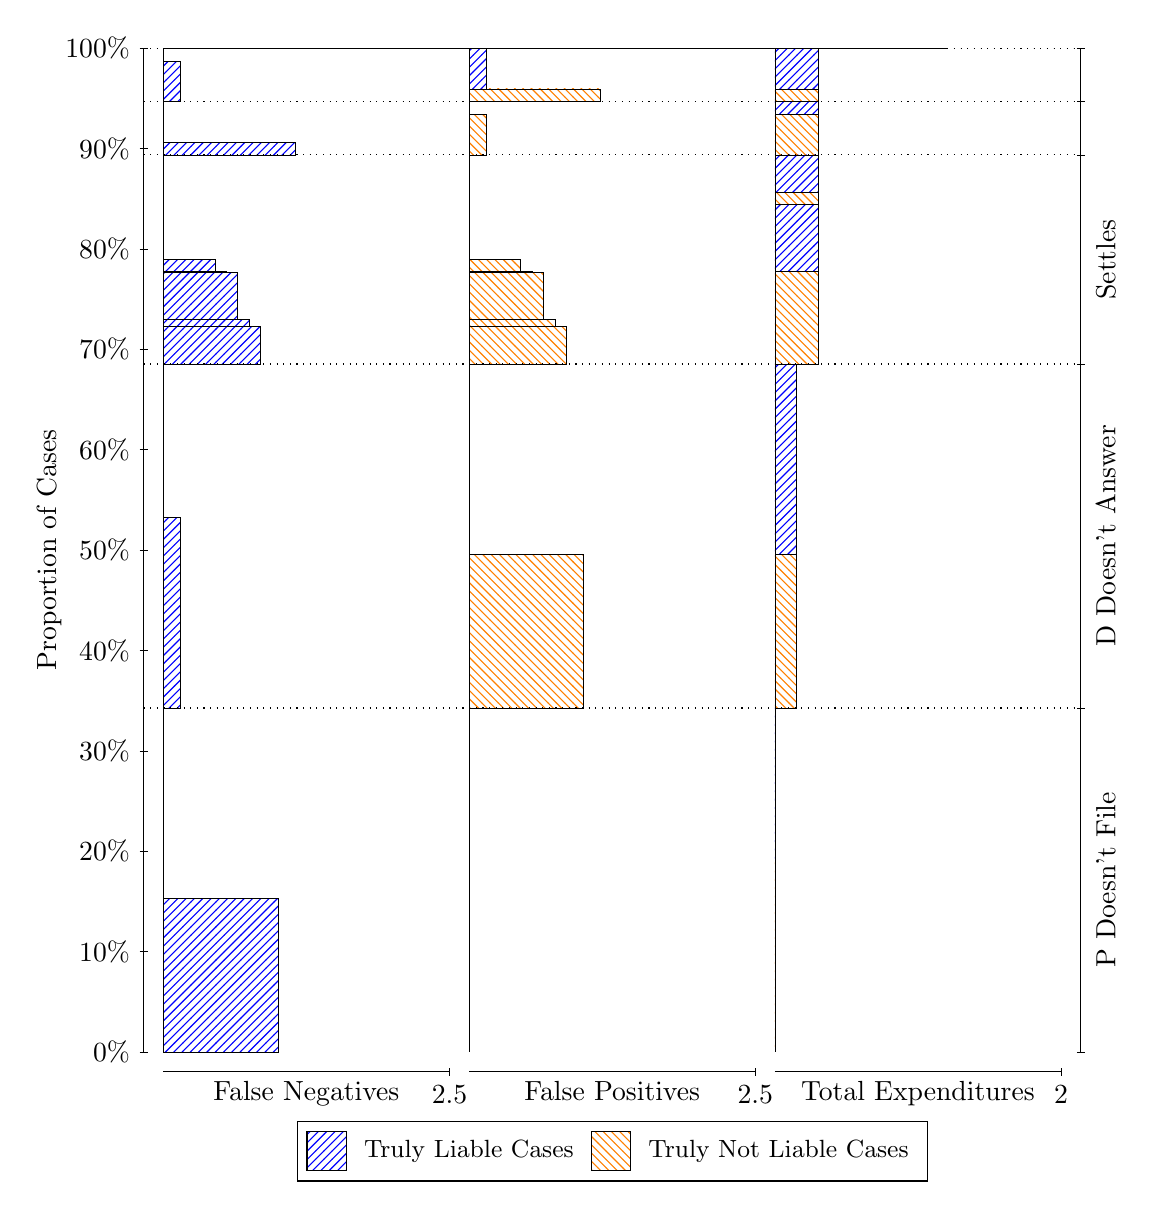
\begin{tikzpicture}
\draw[black, very thin] (1.5,1.75) -- (1.5,14.5);
\node[rotate=90, text=black, anchor=center] at (0.3, 8.125) {Proportion of Cases};
\draw[black, very thin] (1.45,1.75) -- (1.55,1.75);
\node[text=black, anchor=east] at (1.45, 1.75) {0\%};
\draw[black, very thin] (1.45,3.025) -- (1.55,3.025);
\node[text=black, anchor=east] at (1.45, 3.025) {10\%};
\draw[black, very thin] (1.45,4.3) -- (1.55,4.3);
\node[text=black, anchor=east] at (1.45, 4.3) {20\%};
\draw[black, very thin] (1.45,5.575) -- (1.55,5.575);
\node[text=black, anchor=east] at (1.45, 5.575) {30\%};
\draw[black, very thin] (1.45,6.85) -- (1.55,6.85);
\node[text=black, anchor=east] at (1.45, 6.85) {40\%};
\draw[black, very thin] (1.45,8.125) -- (1.55,8.125);
\node[text=black, anchor=east] at (1.45, 8.125) {50\%};
\draw[black, very thin] (1.45,9.4) -- (1.55,9.4);
\node[text=black, anchor=east] at (1.45, 9.4) {60\%};
\draw[black, very thin] (1.45,10.675) -- (1.55,10.675);
\node[text=black, anchor=east] at (1.45, 10.675) {70\%};
\draw[black, very thin] (1.45,11.95) -- (1.55,11.95);
\node[text=black, anchor=east] at (1.45, 11.95) {80\%};
\draw[black, very thin] (1.45,13.225) -- (1.55,13.225);
\node[text=black, anchor=east] at (1.45, 13.225) {90\%};
\draw[black, very thin] (1.45,14.5) -- (1.55,14.5);
\node[text=black, anchor=east] at (1.45, 14.5) {100\%};

\draw[black, very thin] (13.4,1.75) -- (13.4,14.5);
\draw[black, very thin] (13.35,1.75) -- (13.45,1.75);
\node[anchor=west] at (13.35, 1.75) {};
\draw[black, very thin] (13.35,6.1186) -- (13.45,6.1186);
\node[anchor=west] at (13.35, 6.1186) {};
\draw[black, very thin] (13.35,10.487) -- (13.45,10.487);
\node[anchor=west] at (13.35, 10.487) {};
\draw[black, very thin] (13.35,13.143) -- (13.45,13.143);
\node[anchor=west] at (13.35, 13.143) {};
\draw[black, very thin] (13.35,13.819) -- (13.45,13.819);
\node[anchor=west] at (13.35, 13.819) {};
\draw[black, very thin] (13.35,14.495) -- (13.45,14.495);
\node[anchor=west] at (13.35, 14.495) {};
\draw[black, very thin] (13.35,14.498) -- (13.45,14.498);
\node[anchor=west] at (13.35, 14.498) {};
\draw[black, very thin] (13.35,14.5) -- (13.45,14.5);
\node[anchor=west] at (13.35, 14.5) {};

\draw[black, very thin, pattern color=blue, pattern=north east lines] (1.75,1.75) rectangle (3.2033,3.6963);
\draw[black, very thin, pattern color=orange, pattern=north west lines] (1.75,3.6963) rectangle (1.75,6.1186);
\draw[black, very thin, pattern color=blue, pattern=north east lines] (1.75,6.1186) rectangle (1.968,8.5409);
\draw[black, very thin, pattern color=orange, pattern=north west lines] (1.75,8.5409) rectangle (1.75,10.487);
\draw[black, very thin, pattern color=blue, pattern=north east lines] (1.75,10.487) rectangle (2.9853,10.965);
\draw[black, very thin, pattern color=blue, pattern=north east lines] (1.75,10.965) rectangle (2.84,11.053);
\draw[black, very thin, pattern color=blue, pattern=north east lines] (1.75,11.053) rectangle (2.6947,11.653);
\draw[black, very thin, pattern color=blue, pattern=north east lines] (1.75,11.653) rectangle (2.5493,11.664);
\draw[black, very thin, pattern color=blue, pattern=north east lines] (1.75,11.664) rectangle (2.404,11.815);
\draw[black, very thin, pattern color=orange, pattern=north west lines] (1.75,11.815) rectangle (1.75,13.143);
\draw[black, very thin, pattern color=blue, pattern=north east lines] (1.75,13.143) rectangle (3.4213,13.306);
\draw[black, very thin, pattern color=orange, pattern=north west lines] (1.75,13.306) rectangle (1.75,13.819);
\draw[black, very thin, pattern color=blue, pattern=north east lines] (1.75,13.819) rectangle (1.968,14.333);
\draw[black, very thin, pattern color=orange, pattern=north west lines] (1.75,14.333) rectangle (1.75,14.495);
\draw[black, very thin, pattern color=blue, pattern=north east lines] (1.75,14.495) rectangle (5.8193,14.496);
\draw[black, very thin, pattern color=orange, pattern=north west lines] (1.75,14.496) rectangle (1.75,14.498);
\draw[black, very thin, pattern color=orange, pattern=north west lines] (1.75,14.498) rectangle (1.75,14.498);
\draw[black, very thin, pattern color=blue, pattern=north east lines] (1.75,14.498) rectangle (1.75,14.5);
\draw[black, very thin, pattern color=orange, pattern=north west lines] (5.6333,1.75) rectangle (5.6333,4.1723);
\draw[black, very thin, pattern color=blue, pattern=north east lines] (5.6333,4.1723) rectangle (5.6333,6.1186);
\draw[black, very thin, pattern color=orange, pattern=north west lines] (5.6333,6.1186) rectangle (7.0867,8.065);
\draw[black, very thin, pattern color=blue, pattern=north east lines] (5.6333,8.065) rectangle (5.6333,10.487);
\draw[black, very thin, pattern color=orange, pattern=north west lines] (5.6333,10.487) rectangle (6.8687,10.964);
\draw[black, very thin, pattern color=orange, pattern=north west lines] (5.6333,10.964) rectangle (6.7233,11.053);
\draw[black, very thin, pattern color=orange, pattern=north west lines] (5.6333,11.053) rectangle (6.578,11.654);
\draw[black, very thin, pattern color=orange, pattern=north west lines] (5.6333,11.654) rectangle (6.4327,11.664);
\draw[black, very thin, pattern color=orange, pattern=north west lines] (5.6333,11.664) rectangle (6.2873,11.815);
\draw[black, very thin, pattern color=blue, pattern=north east lines] (5.6333,11.815) rectangle (5.6333,13.143);
\draw[black, very thin, pattern color=orange, pattern=north west lines] (5.6333,13.143) rectangle (5.8513,13.657);
\draw[black, very thin, pattern color=blue, pattern=north east lines] (5.6333,13.657) rectangle (5.6333,13.819);
\draw[black, very thin, pattern color=orange, pattern=north west lines] (5.6333,13.819) rectangle (7.3047,13.982);
\draw[black, very thin, pattern color=blue, pattern=north east lines] (5.6333,13.982) rectangle (5.8513,14.495);
\draw[black, very thin, pattern color=orange, pattern=north west lines] (5.6333,14.495) rectangle (5.6333,14.497);
\draw[black, very thin, pattern color=blue, pattern=north east lines] (5.6333,14.497) rectangle (5.6333,14.498);
\draw[black, very thin, pattern color=orange, pattern=north west lines] (5.6333,14.498) rectangle (9.7027,14.498);
\draw[black, very thin, pattern color=blue, pattern=north east lines] (5.6333,14.498) rectangle (8.2493,14.5);
\draw[black, very thin, pattern color=orange, pattern=north west lines] (9.5167,1.75) rectangle (9.5167,4.1723);
\draw[black, very thin, pattern color=blue, pattern=north east lines] (9.5167,4.1723) rectangle (9.5167,6.1186);
\draw[black, very thin, pattern color=orange, pattern=north west lines] (9.5167,6.1186) rectangle (9.7892,8.065);
\draw[black, very thin, pattern color=blue, pattern=north east lines] (9.5167,8.065) rectangle (9.7892,10.487);
\draw[black, very thin, pattern color=orange, pattern=north west lines] (9.5167,10.487) rectangle (10.062,11.664);
\draw[black, very thin, pattern color=blue, pattern=north east lines] (9.5167,11.664) rectangle (10.062,12.514);
\draw[black, very thin, pattern color=orange, pattern=north west lines] (9.5167,12.514) rectangle (10.062,12.666);
\draw[black, very thin, pattern color=blue, pattern=north east lines] (9.5167,12.666) rectangle (10.062,13.143);
\draw[black, very thin, pattern color=orange, pattern=north west lines] (9.5167,13.143) rectangle (10.062,13.657);
\draw[black, very thin, pattern color=blue, pattern=north east lines] (9.5167,13.657) rectangle (10.062,13.819);
\draw[black, very thin, pattern color=orange, pattern=north west lines] (9.5167,13.819) rectangle (10.062,13.982);
\draw[black, very thin, pattern color=blue, pattern=north east lines] (9.5167,13.982) rectangle (10.062,14.495);
\draw[black, very thin, pattern color=orange, pattern=north west lines] (9.5167,14.495) rectangle (11.697,14.497);
\draw[black, very thin, pattern color=blue, pattern=north east lines] (9.5167,14.497) rectangle (11.697,14.498);
\draw[black, very thin, pattern color=orange, pattern=north west lines] (9.5167,14.498) rectangle (11.697,14.498);
\draw[black, very thin, pattern color=blue, pattern=north east lines] (9.5167,14.498) rectangle (11.697,14.5);
\draw[black, dotted] (1.5,6.1186) -- (13.4,6.1186);
\draw[black, dotted] (1.5,10.487) -- (13.4,10.487);
\draw[black, dotted] (1.5,13.143) -- (13.4,13.143);
\draw[black, dotted] (1.5,13.819) -- (13.4,13.819);
\draw[black, dotted] (1.5,14.495) -- (13.4,14.495);
\draw[black, dotted] (1.5,14.498) -- (13.4,14.498);
\draw[black, very thin] (1.75,1.5) -- (5.3833,1.5);
\node[text=black, anchor=north] at (3.5667, 1.5) {False Negatives};
\draw[black, very thin] (5.3833,1.45) -- (5.3833,1.55);
\node[text=black, anchor=north] at (5.3833, 1.45) {2.5};

\draw[black, very thin] (5.6333,1.5) -- (9.2667,1.5);
\node[text=black, anchor=north] at (7.45, 1.5) {False Positives};
\draw[black, very thin] (9.2667,1.45) -- (9.2667,1.55);
\node[text=black, anchor=north] at (9.2667, 1.45) {2.5};

\draw[black, very thin] (9.5167,1.5) -- (13.15,1.5);
\node[text=black, anchor=north] at (11.333, 1.5) {Total Expenditures};
\draw[black, very thin] (13.15,1.45) -- (13.15,1.55);
\node[text=black, anchor=north] at (13.15, 1.45) {2};

\node[text=black, centered, rotate=90] at (13.72, 3.9343) {P Doesn't File};
\node[text=black, centered, rotate=90] at (13.72, 8.3029) {D Doesn't Answer};
\node[text=black, centered, rotate=90] at (13.72, 11.815) {Settles};





\draw (7.449999999999999,1.5) node[draw=none] (baseCoordinate) {};
\begin{scope}[align=center]
        \matrix[scale=0.5, draw=black, below=0.5cm of baseCoordinate, nodes={draw}, column sep=0.1cm]{
            \node[rectangle, draw, minimum width=0.5cm, minimum height=0.5cm, pattern color=blue, pattern=north east lines] {}; &
            \node[draw=none, font=\small, text=black] (B) {Truly Liable Cases}; &
            \node[rectangle, draw, minimum width=0.5cm, minimum height=0.5cm, pattern color=orange, pattern=north west lines] {}; &
            \node[draw=none, font=\small, text=black] (B) {Truly Not Liable Cases}; \\
            };
\end{scope}

\end{tikzpicture}
\end{document}